\begin{apendicesenv}
      
    \partapendices

    %Corrigir erro da numeração dos apendices
    \setcounter{chapter}{0}
    \renewcommand{\thechapter}{\Alph{chapter}}%

    \chapter{Gustavo Lopes}

    O que eu achei de Haskell? Como um usuário de longa data de linguagens orientadas a objeto(OOP), 
    como Java, C++ e mais recentemente Dart, minha experiência inicial com Haskell foi...
    um pouco estranha. Fiquei muito curioso e até encucado em ver Haskell executar códigos, que em
    outras linguagens precisariam ocupar 50 linhas, em apenas 2 ou 3 linhas, como foi o Quicksort.

    Além disso, lendo sua história, achei extremamente fascinante toda a concepção do Haskell,
    mas fiquei triste vendo que é muito difícil encontrar muitas pessoas falando sobre essa linguagem, que nasceu 
    do esforço coletivo de vários programadores, mas que hoje não recebe tanto apoio como outras linguagens.

    Por fim, como curiosidade, eu estava procurando sobre como fazer interfaces em C++ quando
    descobri que a \emph{WxWidgets}, uma biblioteca para criar interface cross-platform, também possui 
    sua versão para Haskell, chamada \emph{WxHaskell}.

    \begin{figure}[ht]
      \includegraphics[width =\textwidth]{gebob.png}
      \caption{GeBoP, um jogo de tabuleiro feito em Haskell, usando WxHaskell}
    \end{figure}

    \newpage

    \chapter{Thiago Henriques}
    
    Bom, como posso expressar o que eu senti aprendendo sobre essa nova linguagem? Eu gosto muito das linguagens de alto nível, principalmente Python,
    então no começo devo admitir que senti um certo desafio. Porém, sinto que Haskell conseguiu cumprir o 
    seu propósito e possibilitou a criação de novos.

    Em geral fiquei fascinado como a linguagem foi implementada e a tomada de decisão da equipe com o passar do tempo. A implementação
    possibilitou a adição de diversas funcionalidades únicas da linguagem e facilitou o desenvolvimento mais fluido da mesma.
    Além disso, achei interresante como em alguns códigos de Haskell eram necessário poucas linhas para se executar uma ação, assim
    me lembrando um pouco de Python.

    Eu observei que Haskell possui diversas implementações no mercado e muitos projetos de código aberto que utilizam da linguagem.
    Um dos projetos que eu achei muito interessante foi o Detexify, feito totalmente em Haskell, que tem como objetivo simplificar a 
    busca de símbolos especiais para aqueles que trabalham em \LaTeX. O usuário só precisa desenhar o símbolo em uma caixa e
    o comando será exibido em \LaTeX.
    
    \begin{figure}[ht]
      \centering
      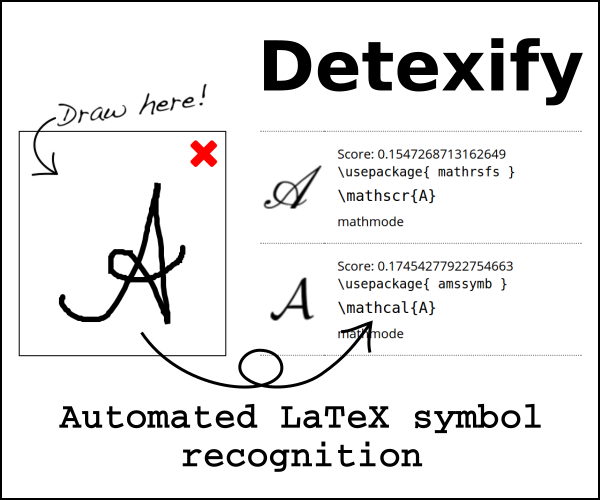
\includegraphics[scale=0.8]{detexify.png}
      \caption{Interface do Detexify}
    \end{figure}

    \newpage 

    \chapter{Lucas Santiago}

    Na minha opinião, Haskell se apresenta de uma forma muito diferente da maioria da outras línguas. 
    Parafraseando Fábio Akita: cada lingua de programação não é mais do que uma ferramenta
    para resolver um problema.

    \begin{figure}[ht]
      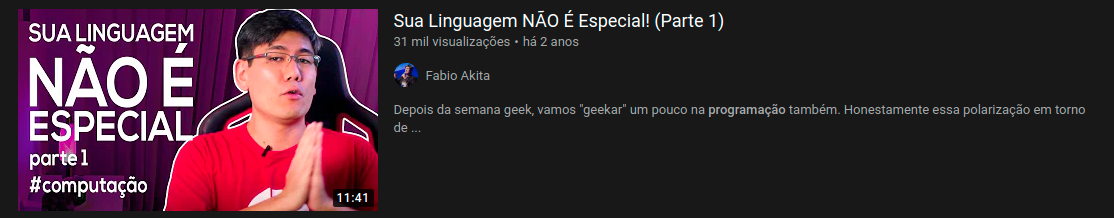
\includegraphics[width =\textwidth]{fabio_akita_lingua.png}
      \caption{\href{https://www.youtube.com/watch?v=p9-WuJbVHHc}{Fabio Akita explicando que linguas de programação são apenas feitas para resolver problemas!}}
    \end{figure}

    Os problemas que Haskell se propôs a resolver são cálculos matemáticos
    funcionais. O paradigma funcional dessa linguagem torna ela bem resistente a efeitos colaterais. Além de ser uma lingua
    \emph{cross-platform}, extremamente importante para todas aquelas pessoas que precisem de uma lingua que funcione
    em qualquer sistema operacional. 

    Como um programador de C/C++ e Python, vejo que Haskell está em um nível intermediário entre essas línguas.
    É interessante ver uma lingua de alto nível com tipagem estática, torna o código bem estável - chances baixas de 
    resultar em erros -, tipagem é fundamental quando se quer garantir precisão de valores nos cálculos.

    Concluindo, não foi tão intuitivo aprender Haskell, ele possui várias propriedades que não existem em nenhuma das línguas
    que conhecia. Entretando, isso foi extremamente positivo para mim, aprendi várias coisas novas. Abaixo há
    mais um vídeo do Fabio Akita, dessa vez citando que nem sempre é fácil aprender algo novo. Em programação,
    quando você aprende da forma correta, várias novas possibilidades de resolução de problemas começam a aparecer.

    \begin{figure}[ht]
      \includegraphics[width =\textwidth]{fabio_akita_programar_eh_dificil.png}
      \caption{\href{https://www.youtube.com/watch?v=V7oUDL7E1g4}{Fabio Akita explicando que programação nem sempre é fácil.}}
    \end{figure}

    \newpage

    \chapter{Pedro Souza}

    Haskell definitivamente é uma linguagem um tanto quanto diferente das outras que são consideradas mais comuns Java, C++, C\#, Javascript,
    Python, etc. Apesar de não ter uma sintaxe muito complexa, sua implementação pode ser um pouco estranhada para quem está começando a conhecer
    a linguagem. 

    O fato de ser baseada em expressões, Haskell se torna um tanto quanto amedrontador para programadores novos, com pouca experiência e que estão
    mais acostumados com as linguagens mais usuais. Apesar de ter estudado e descoberto um pouco mais sobre a linguagem, admito que continuo 
    relutante quanto a usá-la. Talvez por ser um programador ainda em formação e com pouca experiência, não consigo ainda pensar em aplicações 
    que necessariamente teriam de ser feitas com Haskell.

    Como muitas outras linguagens por aí, Haskell continua muito oculta, sem muito reconhecimento e fama, um grande exemplo disso é que se pesquisarmos
    ``Haskell'' no google, encontraremos algum resultado sobre a linguagem apenas na segunda página e no último item encontrado. E aqui entre nós, quantas vezes vamos
    até a segunda página do google em alguma pesquisa?

    \begin{figure}[ht]
        \centering 
        \includegraphics[scale=0.3]{Haskellgoogle.png}
        \caption{Haskell, linguagem de programação apenas no último item da segunda página do google}
    \end{figure}

\end{apendicesenv}